\documentclass[12pt]{article}

\usepackage[margin=1in]{geometry}  % set the margins to 1in on all sides
\usepackage{graphicx}              % to include figures
\usepackage{amsmath}               % great math stuff
\usepackage{amsfonts}              % for blackboard bold, etc
\usepackage{amsthm}                % better theorem environments
\usepackage{url}

% various theorems, numbered by section

\newtheorem{thm}{Theorem}[section]
\newtheorem{lem}[thm]{Lemma}
\newtheorem{prop}[thm]{Proposition}
\newtheorem{cor}[thm]{Corollary}
\newtheorem{conj}[thm]{Conjecture}
\newtheorem{dfn}[thm]{Definition}

\DeclareMathOperator{\id}{id}

\newcommand{\bd}[1]{\mathbf{#1}}  % for bolding symbols
\newcommand{\RR}{\mathbb{R}}      % for Real numbers
\newcommand{\ZZ}{\mathbb{Z}}      % for Integers
\newcommand{\col}[1]{\left[\begin{matrix} #1 \end{matrix} \right]}
\newcommand{\comb}[2]{\binom{#1^2 + #2^2}{#1+#2}}
	

\begin{document}


\nocite{*}

\title{A Generalized Sphere Theorem for Positively Curved Combinatorial 3-Manifolds}

\author{Aaron Trout \\ Department of Mathematics \\
Chatham University \\ Woodland Rd, Pittsburgh PA 15232 USA \and
Vadas Gintautas\\ Department of Physics \\
Chatham University \\ Woodland Rd, Pittsburgh PA 15232 USA}


\maketitle

\begin{abstract}
  This paper presents a discrete version of Grove and Shiohama's generalized sphere theorem \cite{groveshiohama}.
\end{abstract}


\section{Introduction}

Differential geometry is of central importance not only to geometers but also topologists, physicists and, increasingly, many of those interested in applied topics such as finite element analysis and computer graphics. One new offshoot in this area is {\em discrete differential geometry} (DDG) which seeks discrete analogues to the classical theorems and concepts from differential geometry. Since many computational treatments of differential geometry involve discretizing shapes, this subject has particular relevance for those with applied interests \cite{grinspun2006discrete}. Other recent DDG work can be found in \cite{BMM,Crowley,EMM,forman2,GGL1,GGL2,GGL3,stone}. 

A particularly important goal in classical differential geometry is to elucidate the relationship between the curvature of a Riemannian (or semi-Riemannian) space and its topology. The classical
results in this area are numerous, beautiful, and have inspired an
enormous amount of subsequent research. In this paper, we will present a discrete analogue of the ``generalized'' sphere theorem of Grove and Shiohama \cite{groveshiohama}.

\begin{thm}[Grove-Shiohama] Let $M$ be a complete, connected, $n$-dimensional Riemannian manifold with section curvature $K \geq \delta > 0$ and diameter greater than $\frac{\pi}{2\sqrt{\delta}}$. Then, $M$ is homeomorphic to a sphere.
\label{thm:grove_shiohama}
\end{thm}

\noindent Note that this bound is sharp, since the real projective space $\mathbb{RP}^n$ admits a metric with uniform sectional curvature $K=1$ and diameter $\pi/2$. We should also note also that the diameter bound in Theorem \ref{thm:gove_shiohama} is exactly half the maximum diameter allowed by the Bonnet-Myers theorem:

\begin{thm}[Bonnet-Myers] Let $M$ be a complete, connected, $n$-dimensional Riemannian manifold with section curvature $K \geq \delta > 0$. Then the diameter of $M$ is at most $\frac{\pi}{\sqrt{\delta}}$.
\label{thm:bonnet_myers}
\end{thm}

\noindent Our results are derived from brute-force checking of a combinatorial 3-manifold census created by Lutz and Sullivan \cite{LS}.

\section{Basic Stuff}
\label{sect:basics}

The discrete version of Theorem \ref{thm:grove_shiohama} given in this paper will apply to positively curved combinatorial 3-manifolds. A {\em combinatorial 3-manifold} is an abstract simplicial complex in which the link of each vertex is a 2-sphere. We call such a space {\em positively curved} if at most five tetrahedra are incident along each edge. Why this terminology? If we endow a combinatorial 3-manifold with the standard piecewise-linear (PL) metric (in which all edges have unit-length), this condition is equivalent to requiring an angle deficit along each edge. In classical differential geometry an angle deficit is intimately related to positive curvature.

Probably the most natural discrete definition of distance in an abstract simplicial complexe is given in terms of edge paths.

\begin{dfn}The {\em edge-distance} between two vertices $v$ and $w$ in an abstract simplicial complex $M$ is the minimum length, in edges, of an edge path from $v$ to $w$. We denote this quantity $d_1(v,w)$. The {\em edge-diameter} of $M$, written as $diam_1(M)$, is the maximum of $d_1(v,w)$ over all pairs of vertices $v$ and $w$ in $M$. 
\end{dfn}

\noindent Previous work \cite{Trout10} has demonstrated a discrete version of the Bonnet-Myers theorem which applies to positively curved combinatorial 3-manifolds and which uses these notions of distance and diameter.

\begin{thm}[Trout] For any positively curved combinatorial 3-manifold $M$ we have $diam_1(M)\leq 5$. Moreover, this bound is sharp.
\label{thm:discrete_BM}
\end{thm}

While Theorem \ref{thm:discrete_BM} is stated in terms of edge-diameter, the proof is greatly facilitated by expanding the set of paths under consideration to include those which contain not only edges, but also other types of PL-paths between vertices. The first new type of path is called a {\em hop}.

\begin{dfn}[Hops] Suppose $\tau$ is a 2-simplex in $M$ and $v_1$ and $v_2$ vertices in $M$ such that $v_1*\tau$ and $v_2*\tau$ are 3-simplices in $M$. The PL-path from $v_1$ through the barycenter of $\tau$ and ending on $v_2$ will be called a {\em hop} from $v_1$ to $v_2$. See Figure \ref{hop}. TO DO: WHY DOES THIS SAY FIGURE 2?!?!
\end{dfn}

\noindent The other new type of path we call a {\em jump.}

\begin{dfn}[Jumps] Suppose there are edges $e_1$ and $e_2$ and vertices $v_1$ and $v_2$ in $M$ so that $e_1*e_2$ is a 3-simplex in $M$ and $v_1*e_1$ and $v_2*e_2$ are 2-simplices in $M$. We call the PL-path from $v_1$ through the barycenters of $e_1$ and $e_2$ and ending on $v_2$ a {\em jump} from $v_1$ to $v_2$. See Figure \ref{jump}.
\end{dfn}

\noindent The length of each hop and edge will be its length as a PL-path in the standard PL metric. Some basic Euclidean geometry tells us these lengths are $H = \frac{2}{3}\sqrt{2}$ and $J = \frac{1}{2}\sqrt{2} + \sqrt{3}$ respectively. We let $d(v,w)$ denote the distance between vertices $v$ and $w$ obtained by minimizing over all paths containing edges as well as hops and jumps. Similarly, we let $diam(M)$ denote the diameter defined in terms of this new distance.

Why are these paths relevant to this paper? The classical generalized sphere theorem requires the manifold to have diameter more than half the maximum allowed by the Bonnet-Myers theorem. If we were to naively imitate the discrete Bonnet-Myers result, Theorem \ref{thm:discrete_BM}, the corresponding diameter inequality would be $diam_1(M)>2.5$. Since only integral values of edge-distance can occur, this would correspond to $diam(M)\geq 3$. Unfortunately, this bound will not work since there are triangulations of $\mathbb{RP}^3$ with edge-diameter three. However, if we instead use the finer-grained measure of diameter, $diam(M)$ this problem disappears. 
 
\begin{figure}
	\label{hop}
    \begin{center}
        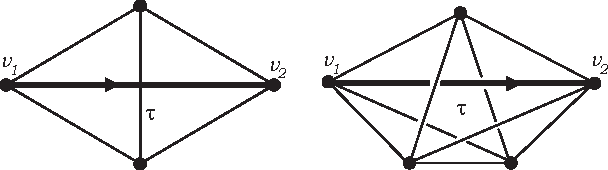
\includegraphics[width=0.6\linewidth]{figures/hops.pdf}
        \caption{A {\em hop} from vertex $v_1$ to vertex $v_2$. TO DO: CROP OUT LEFT IMAGE}
    \end{center}
\end{figure}

\begin{figure}
    \label{jump}
    \begin{center}
        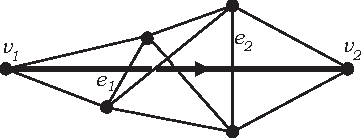
\includegraphics[width=0.4\linewidth]{figures/jump.pdf}
        \caption{A {\em jump} from vertex $v_1$ to vertex $v_2$}
    \end{center}
\end{figure}

\section{Results}

diameter statistics by topological type

\begin{tabular} {| l l | l l | l l | l l | l l |}
\hline
\multicolumn{2}{|c|}{$S^{3}/Q$} &
\multicolumn{2}{|c|}{$L(3,1)$} &
\multicolumn{2}{|c|}{$RP^{3}$} &
\multicolumn{2}{|c|}{$S^{3}$} &
\multicolumn{2}{|c|}{$L(4,1)$} \\
\hline
\hline
$1H$&1    &$2E$&1    &$1H$&10    &$1E$&3    &$1J$&1 \\
  &       &$1J$&1    &$2E$&7     &$1H$&173  &    &  \\
  &       &  &       &$1J$&5     &$2E$&401  &    &  \\
  &       &  &       &    &      &$1J$&2438 &    &  \\
  &       &  &       &    &      &$3E$&1060 &    &  \\
  &       &  &       &    &      &$2H$&582  &    &  \\
  &       &  &       &    &      &$4E$&93   &    &  \\
  &       &  &       &    &      &$2J$&11   &    &  \\
\hline
\end{tabular}

global diameter statistics by topological type

\begin{tabular} {| l l |}
\hline
$1E$ &       3\\
$1H$ &       184\\
$2E$ &       409\\
$1J$ &       2445\\
$3E$ &       1060\\
$2H$ &       582\\
$4E$ &       93\\
$2J$ &       11\\
\hline
\end{tabular}


\begin{figure}
    \begin{center}
    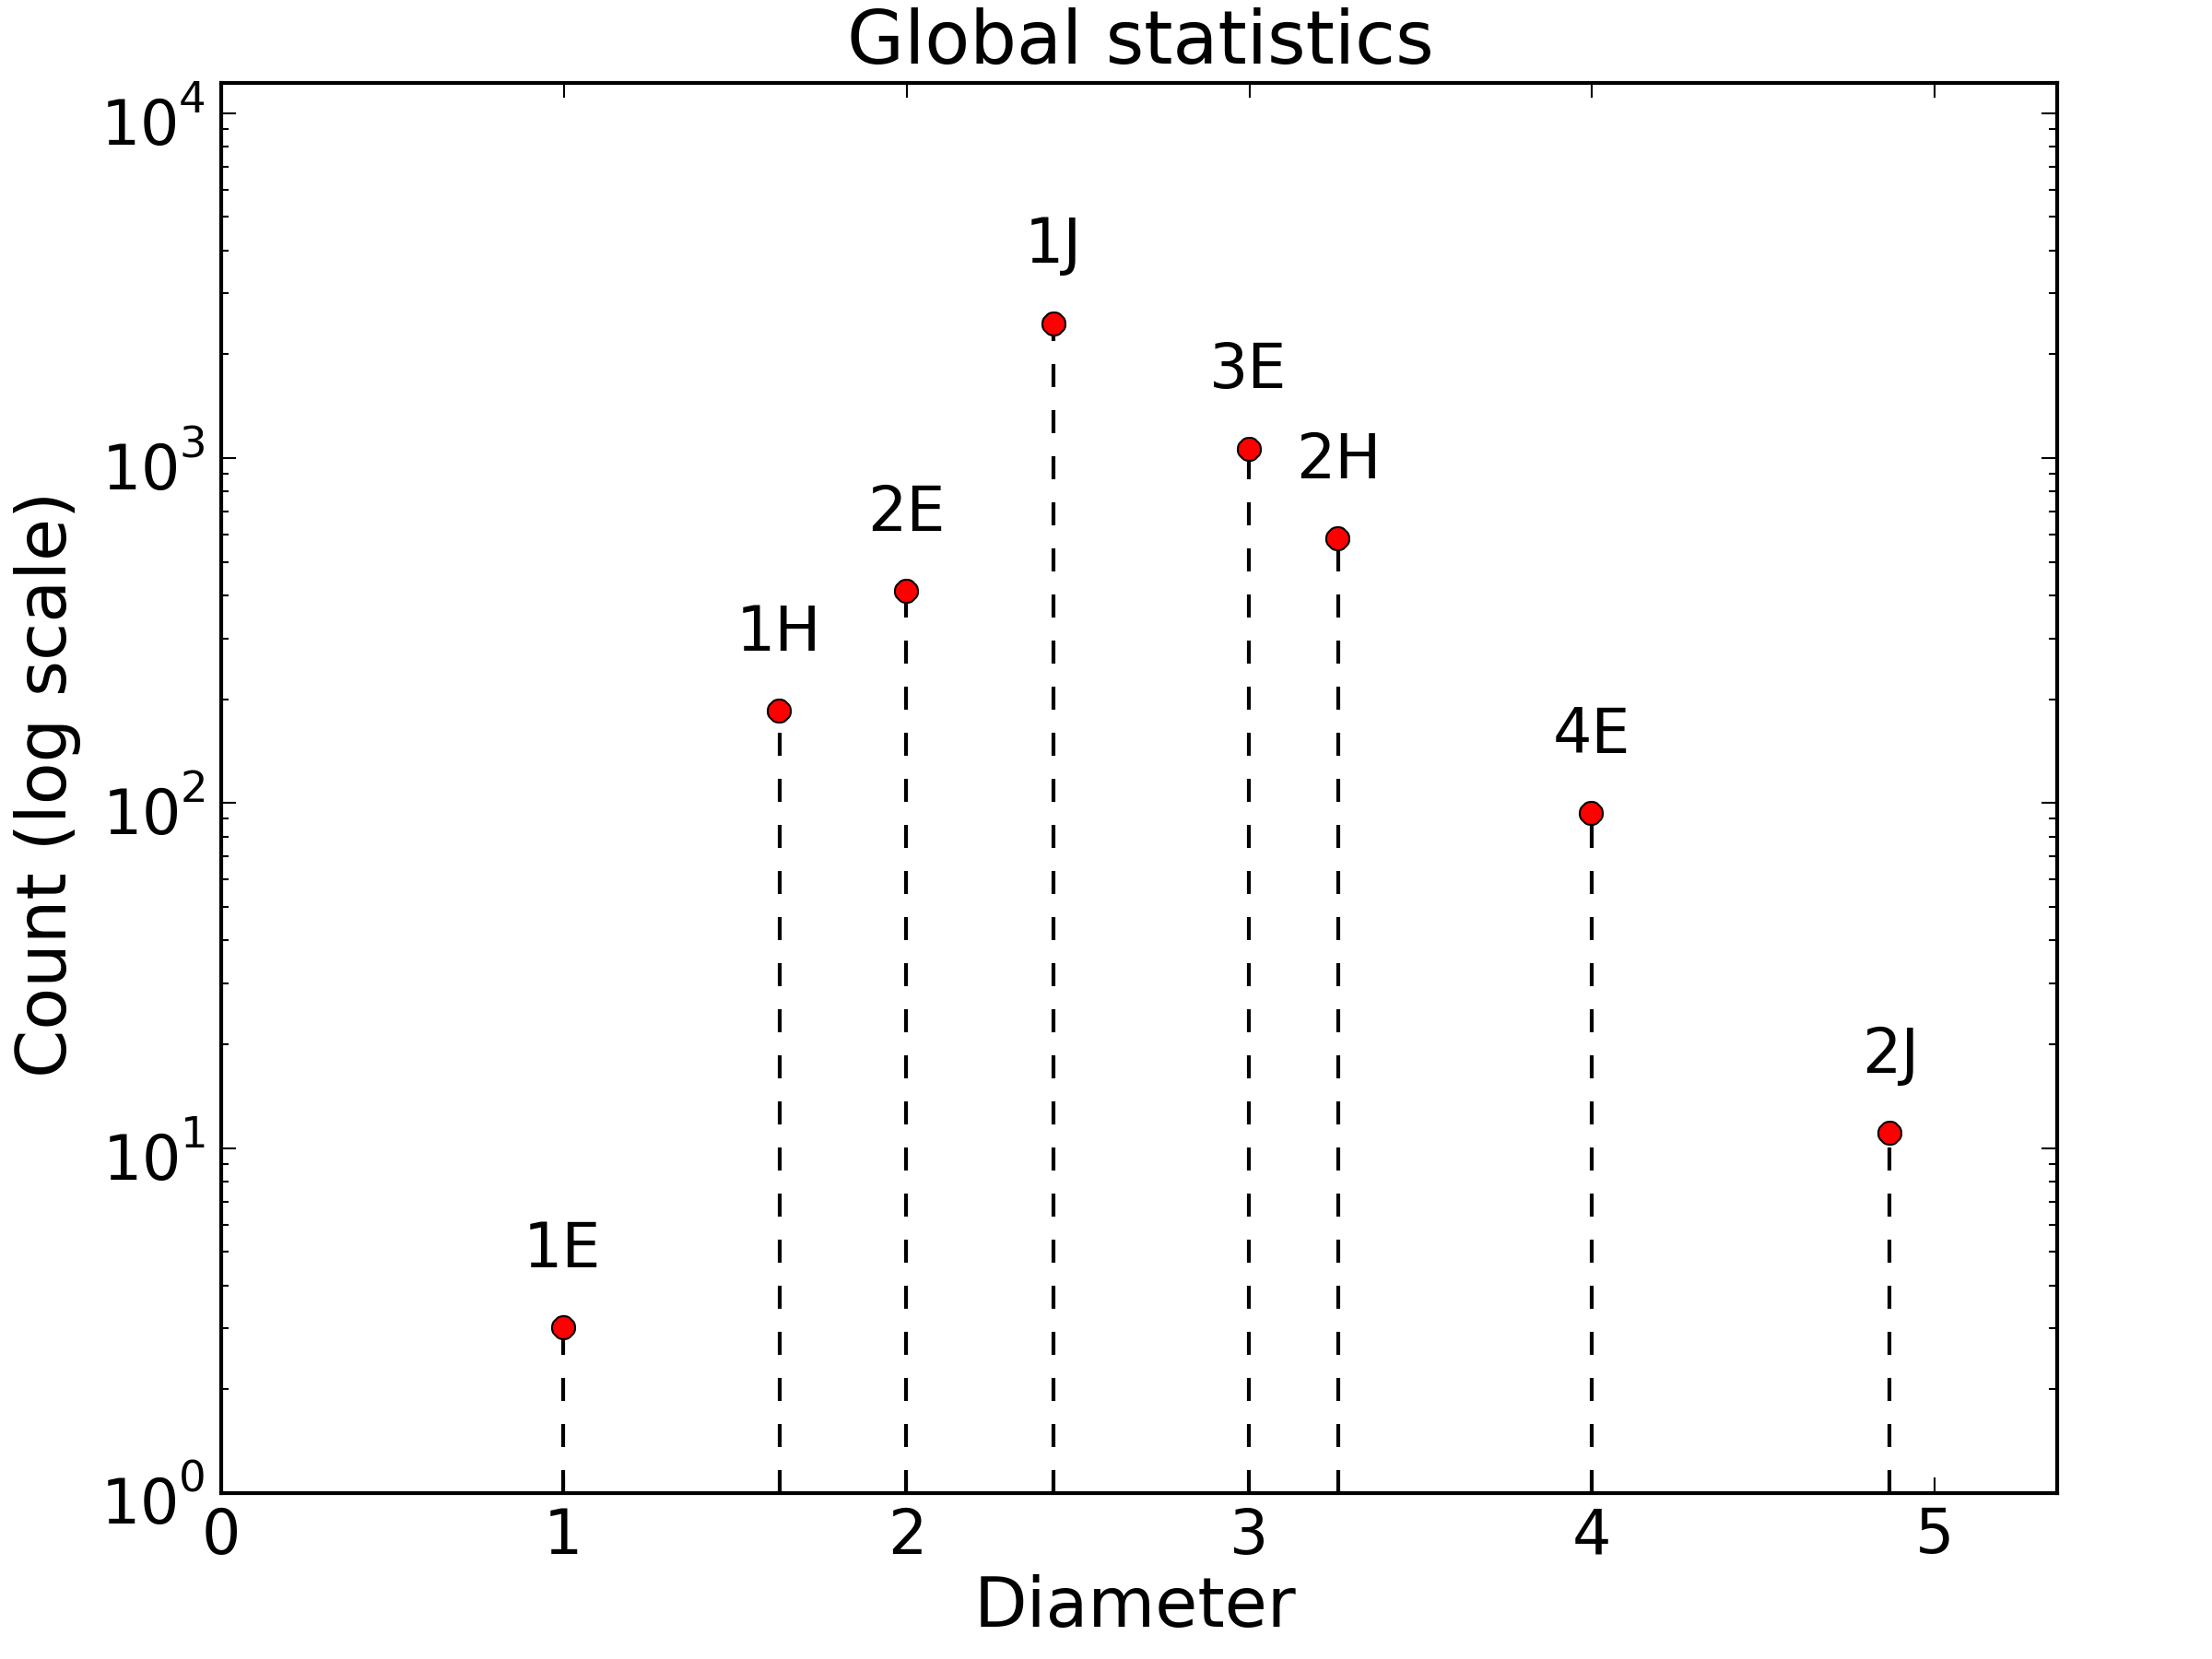
\includegraphics[width=0.6\linewidth]{figures/global_statistics.png}
    \caption{Global statistics}
    \end{center}
    \label{global_statistics}
\end{figure}

\bibliographystyle{plain}
\bibliography{manifolds}
\end{document}
